All the algorithms have been runned 10 times with same data and the same conditions. Figures \ref{fig:users_operations_2g_report} and \ref{fig:users_operations_1t_big} p.\pageref{fig:users_operations_2g_report} shows the total number of users operations.

%\begin{figure}
%	\center
%  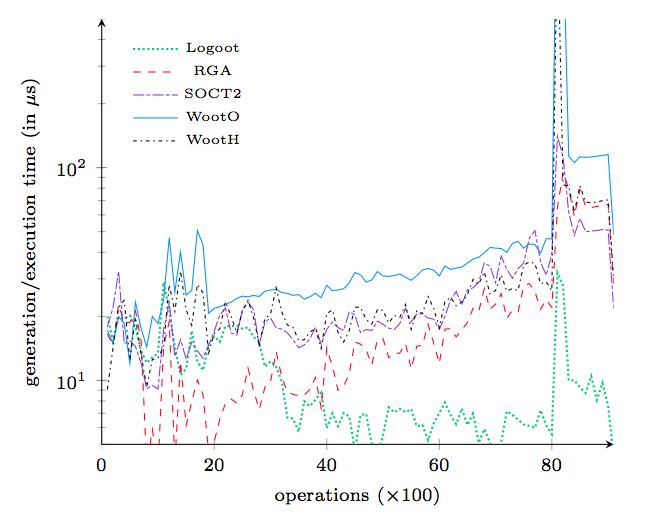
\includegraphics[width=0.6\textwidth]{includes/users_operations_1t_big.png}
%  \caption{User operation execution times - 1st series}
%  \label{fig:users_operations_1t_big}
%\end{figure}  
%\begin{figure}
%	\center
%  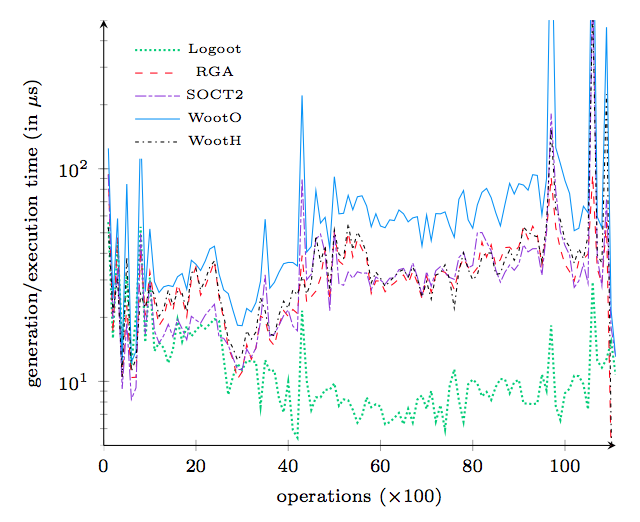
\includegraphics[width=0.6\textwidth]{includes/users_operations_2g_report.png}
%  \caption{User operation execution times - 2nd group
%report}
%  \label{fig:users_operations_2g_report}
%\end{figure}

\begin{figure}[h]

\begin{minipage}{0.50\linewidth}
  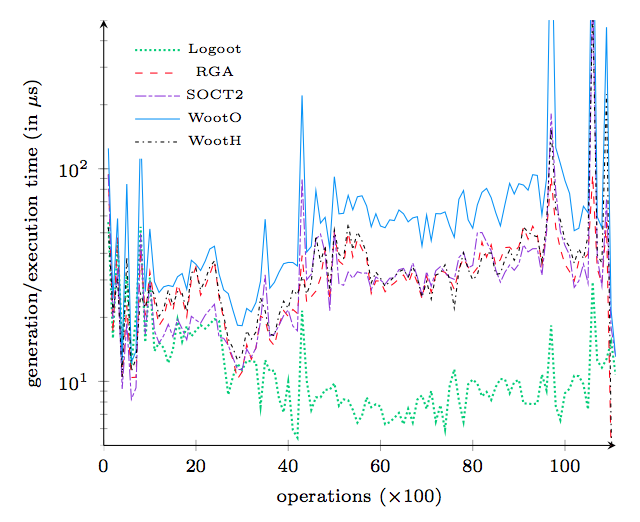
\includegraphics[width=1.2\textwidth]{includes/users_operations_2g_report.png}
  \caption{User operation execution times - 2nd group
report}
  \label{fig:users_operations_2g_report}
  \end{minipage} \hfill
  \begin{minipage}{.50\linewidth}
    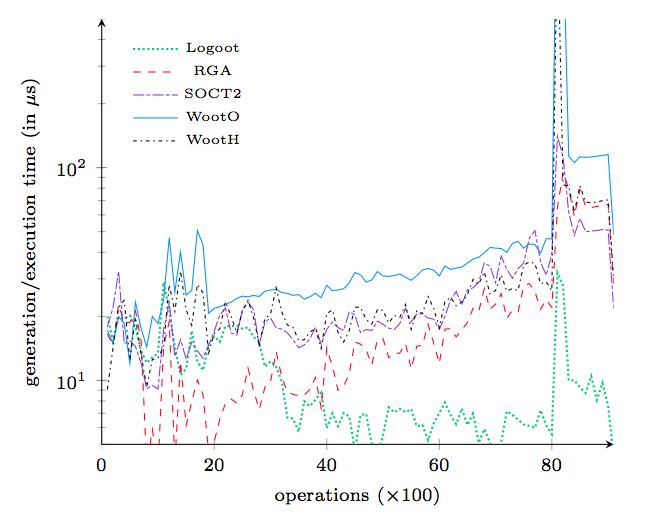
\includegraphics[width=1.2\textwidth]{includes/users_operations_1t_big.png}
  	\caption{User operation execution times - 1st series}
  	\label{fig:users_operations_1t_big}
\end{minipage} \hfill
\end{figure}

The increases are due to insert or delete a large group of characters on the document. All the algorithms decrease over the time because of the size of the document (the unique identifier gets bigger when there are a lot of operations) but logoot decreases slowly compared to the others.\\

Figures \ref{fig:characters_operations_2g_report} and \ref{fig:characters_operations_1t_big} p.\pageref{fig:characters_operations_2g_report} shows the total number of characters operations.

\begin{figure}[h]
\begin{minipage}{0.50\linewidth}
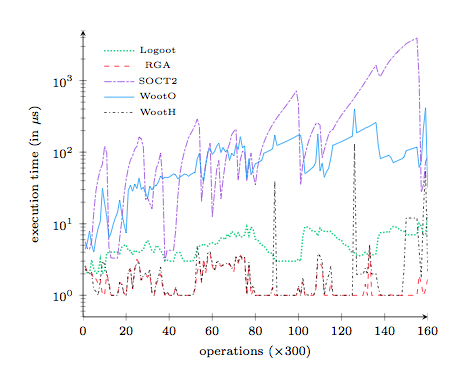
\includegraphics[width=1.2\textwidth]{includes/characters_operations_2g_report.png}
  \caption{Character operation execution times - 2nd
group report}
  \label{fig:characters_operations_2g_report}
  \end{minipage} \hfill
  \begin{minipage}{.50\linewidth}
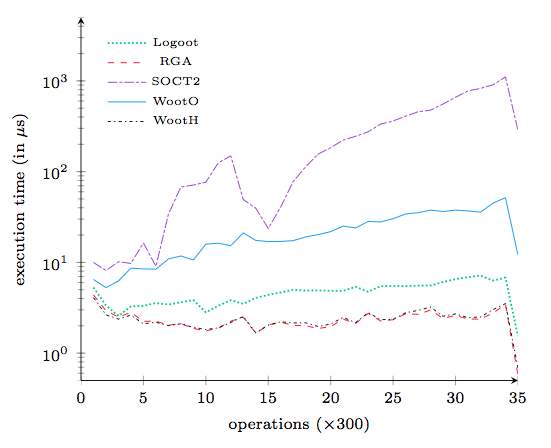
\includegraphics[width=1.2\textwidth]{includes/characters_operations_1t_big.png}
  \caption{Character operation execution times - 1 time
series}
  \label{fig:characters_operations_1t_big}
\end{minipage} \hfill
\end{figure}

Wooto, Logoot and RGA remains stable during al the time. The behavior of SOCT2 performance is mainly due to its garbage collection mechanism. Users have a period of inactivity and the garbage mechanism cannot purge the history log. SOCT2 can't be used for real-time editing because of his response time increasing 50ms quickly.\\

Figure \ref{fig:characters_operations_2g_report} is a bite different than \ref{fig:characters_operations_1t_big} because of the number of characters deletes (students didn't delete as much as in the serie experiments as in the report experiment). RGA and WootH are better than the others because their algorithms are based on hash tables.\\

